\documentclass[../Cours.tex]{subfiles}
\begin{document}

\chapitre{Fractions}

\partie{Concept}

\definition{Soient deux nombres entiers $a$ et $b$, $b \neq 0$.\\Le quotient de $a$ par $b$ est le nombre qui, multiplié par $b$, est égal à $a$.}

\notation{On le note $\dfrac{a}{b}$.}

\renewcommand{\CancelColor}{\color{red}}
\begin{listedexemples}
    \item \fbox{$\dfrac{7}{3}$} : $\dfrac{7}{3} \times 3 = \dfrac{7}{\cancel{3}} \times \cancel{3} = 7$
    \item \fbox{$\dfrac{17}{6}$} : $\dfrac{17}{6} \times 6 = \dfrac{17}{\cancel{6}} \times \cancel{6} = 17$
\end{listedexemples}

\vocabulaire{On dit qu'un nombre est rationnel lorsqu'il peut s'écrire sous forme de fraction.}

\begin{listedexemples}
    \item $\dfrac{3}{4}$ est un nombre rationnel car c'est une fraction.
    \item $1{,}5$ est un nombre rationnel car il peut s'écrire comme une fraction $1,5 = \dfrac{3}{2}$
    \item $1,333...$ est un nombre rationnel car il peut s'écrire sous forme de fraction $1,333... = \dfrac{4}{3}$
    \item $\pi$ n'est pas un nombre rationnel, il n'est pas possible de l'écrire sous forme de fraction.
\end{listedexemples}

\definition{Soient $k$ et $n$ deux nombres entiers ($n$ non nul).\\ Coupons un ensemble en $n$ parts égales et sélectionnons $k$ morceaux partageant une caractéristique commune.\\ La proportion (aussi appelé la fréquence) de cette caractéristique dans cet ensemble sera de $\frac{k}{n}$.}

\begin{listedexemples}
    \item Dans le drapeau de la République Française, il y a 3 morceaux. Parmi ces morceaux, $1$ seul est bleu. La proportion de bleu dans le drapeau tricolore est donc de $\frac{1}{3}$.
    
    \begin{center}
    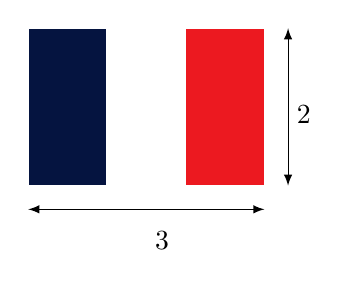
\begin{tikzpicture}
        \definecolor{bleuRF}{RGB}{05, 20, 64}
        \definecolor{blancRF}{RGB}{255, 255, 255}
        \definecolor{rougeRF}{RGB}{236, 25, 32}
        \draw[white, fill=bleuRF] (0,0) rectangle (1,2);
        \draw[white, fill=blancRF] (1,0) rectangle (2,2);
        \draw[white, fill=rougeRF] (2,0) rectangle (3,2);
        \draw[black, latex-latex] (0,-0.3) -- (3,-0.3);
        \draw[black, latex-latex] (3.3,0) -- (3.3,2);
        \node[black] at (1.7,-0.7) {3};
        \node[black] at (3.5,0.9) {2};
    \end{tikzpicture}
    \end{center}
    \item Dans une classe de 35 élèves, il y a 17 filles. Donc la proportion de filles dans la classe est de $\frac{17}{35}$.
    \item 100 personnes sont interrogés pour un sondage. 26 veulent voter pour le candidat A à la prochaine élection. La proportion d'électeurs potentiels du candidat A est de $\frac{26}{100} = 26~\%$.
\end{listedexemples}

\partie{Égalité de fractions}

\definition{Deux fractions sont égales lorsque les divisions qu'elles représentent ont le même quotient.}

\exemple{$\frac{3}{4}$ et $\frac{6}{8}$ sont égales car $3\div 4 = 0,75$ et $6\div 8 = 0,75$.}

\propriete{Soient $a$, $b$, $c$, $d$ et $k$ des nombres entiers. ($b$ et $d$ non nuls, $a < c$ et $b < d$).\\ $\dfrac{a}{b} = \dfrac{c}{d}$ si et seulement s'il existe $k$ tel que $a \times k = c$ et $b \times k = d$.} 

\exemple{$\dfrac{3}{4} = \dfrac{6}{8}$ car je peux multiplier en haut et en bas par $2$.
\begin{center}
\begin{tikzpicture}
    \node at (0,0) {$\dfrac{3}{4} ~~=~~ \dfrac{6}{8}$};
    \coordinate (O) at (0,0);
    \draw[rouge,->] (-0.7,0.6) arc (140:40:1);
    \draw[rouge,->] (-0.7,-0.6) arc (-140:-40:1);
    \node[rouge] at (0,1.2) {$\times 2$};
    \node[rouge] at (0,-1.3) {$\times 2$};
\end{tikzpicture}
\end{center}
}

\propriete{(Reformulation) Multiplier (ou diviser) le numérateur et le dénominateur d'une fraction par le même nombre permet d'obtenir une fraction égale à celle d'origine.}

\definition{Simplifier une fraction signifie trouver une autre fraction égale à la première possédant un numérateur et un dénominateur plus petits.}

\exemple{Je peux simplifier $\frac{9}{12}$ en $\frac{3}{4}$, en divisant le numérateur et le dénominateur par 3.\\
$$\frac{9}{12} = \frac{3 \times 3}{4 \times 3} = \frac{3 \times \cancel{3}}{4 \times \cancel{3}} = \frac{3}{4}$$
Ici, nous pouvons dire que nous avons simplifié par 3.}

\partie{Addition de fractions}

\regle{Soient $a$, $b$, $c$ trois nombres entiers, avec $b \neq 0$. $$\dfrac{a}{b} + \dfrac{c}{b} = \dfrac{a+c}{b}$$}

\remarque{Il faut que les dénominateurs soient égaux pour additionner les fractions.}

\begin{listedexemples}
    \item $\dfrac{2}{3} + \dfrac{4}{3} = $
    \item $\dfrac{4}{7} + \dfrac{3}{7} = $
\end{listedexemples}

\begin{mdframed}
    \centerline{Que faire dans cette situation ?}
    $$ A = \dfrac{2}{3} + \dfrac{7}{18} = ? $$
    \begin{enumerate}
        \item[$\Rightarrow$] On ramène à 18 le dénominateur de la première fraction : $\dfrac{2}{3} = \dfrac{?}{18}$ 
        \item[$\Rightarrow$] On trouve que : $\dfrac{2}{3} = \dfrac{2 \times 6}{3 \times 6} = \dfrac{12}{18}$
        \item[$\Rightarrow$] Finalement, $A = \dfrac{12}{18} + \dfrac{7}{18} = \dfrac{12+7}{18} = \dfrac{19}{18}$
    \end{enumerate}
\end{mdframed}


\end{document}